\begin{center}
	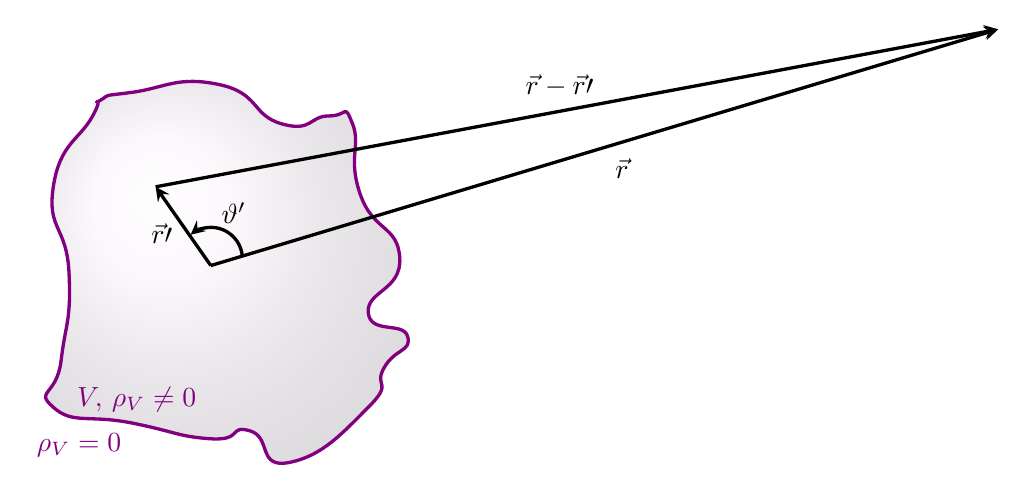
\begin{tikzpicture}[line width = 1.2pt, line join=round,x=1cm,y=1cm,>=stealth]
		% Multipol
		\coordinate (a) at (-1,-2);
		\coordinate (b) at (0,-2.2);
		\coordinate (c) at (0.5,-2.1);
		\coordinate (d) at (1,-2.5);
		\coordinate (e) at (2,-1.8);
		\coordinate (f) at (2.2,-1.3);
		\coordinate (g) at (2.5,-0.9);
		\coordinate (h) at (2,-0.6);
		\coordinate (i) at (2.4,0.1);
		\coordinate (j) at (1.9,0.9);
		\coordinate (k) at (1.8,1.8);
		\coordinate (l) at (1.5,1.9);
		\coordinate (m) at (0.9,1.8);
		\coordinate (n) at (0.1,2.3);
		\coordinate (o) at (-1,2.2);
		\coordinate (p) at (-1.4,2.1);
		\coordinate (q) at (-1.5,1.9);
		\coordinate (r) at (-2,1);
		\coordinate (s) at (-1.8,-0.1);
		\coordinate (t) at (-1.9,-1.2);
		\coordinate (u) at (-2,-1.8);
		\shade[ball color=white!10!violet!20,opacity=0.20] plot [smooth cycle, tension = 1] coordinates {(b) (c) (d) (e) (f) (g) (h) (i) (j) (k) (l) (m) (n) (o) (p) (q) (r) (s) (t) (u) (a)};
		\draw [color=violet] plot [smooth cycle, tension = 1] coordinates {(b) (c) (d) (e) (f) (g) (h) (i) (j) (k) (l) (m) (n) (o) (p) (q) (r) (s) (t) (u) (a)} node [sloped, above] {\ $V,\, \rho_\text{V} \neq 0 $};
		\draw [color=violet] (a) node[anchor=north east] {$ \rho_\text{V} = 0 $};
		% Winkel theta'
		\draw [color=black,->] (10/25,3/25) arc (5:130:10/25);
		\draw [color=black] (0,0.4) node[anchor = south west] {$\vartheta'$};
		% Punkte
		\coordinate (oa) at (10,3);
		\coordinate (ob) at (-0.7,1);
		% Ortsvektor
		\draw [->] (0,0) -- (oa);
		\draw (5,1.5) node[anchor = north west] {$\vec{r} $};
		% Quellvektor
		\draw [->] (0,0) -- (ob);
		\draw (-0.35,0.4) node[anchor = east] {$ \vec{r}\prime  $};
		% Abstandsvektor
		\draw [->,color=black] (ob) -- (oa);
		\draw [color=black] (5,2) node[anchor=south east] {$\vec{r}  - \vec{r}\prime $};
	\end{tikzpicture}
\end{center}